\section{Introduction}
\label{sec:intro}

With the rapid development of intelligent transportation, autonomous driving, and urban management, digital twin technology, as an important innovative tool, has gradually shown tremendous potential in various fields\cite{Alpher17}. 
A digital twin refers to the creation of a digital model corresponding to the real world through the real-time synchronization of data collected from the physical world and virtual models\cite{Alpher20c}. 
This technology can simulate, analyze, and optimize the real world in a virtual environment, thus providing support for decision-making\cite{Alpher21b}. 
In the field of autonomous driving, digital twin technology can accurately replicate factors such as traffic flow, road structure, and pedestrian behavior, providing a precise testing and training environment for the perception, planning, and control of autonomous driving systems\cite{Alpher24}\cite{Alpher20d}.

The focus of this research is to apply digital twin technology to the development and testing of autonomous driving systems to improve the interpretability and robustness of autonomous driving systems by replicating real traffic flow scenarios\cite{Alpher24b}.
By constructing high-precision digital twin models and combining reinforcement learning with simulation platforms, we are able to simulate complex driving scenarios and train and optimize autonomous driving algorithms\cite{Alpher22c}. 
At the same time, digital twin technology can provide smarter decision support for traffic management, promoting the development of smart city construction\cite{Alpher17b}.

\begin{figure}[t]
	\centering
	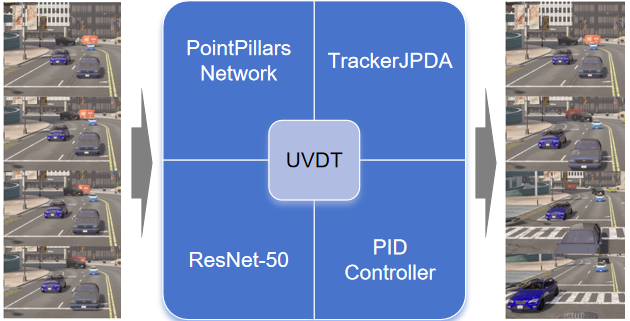
\includegraphics[width=\linewidth]{picture/picture1.png} 
	\caption{Overall Preview of Digital Twin through UVDT} 
	\label{fig:example} 
\end{figure}

We primarily conducted research from four aspects: single-intersection multi-target tracking, multi-intersection multi-target tracking, trajectory inference and restoration, and digital twinning. 
By fusing camera and radar detection, we improved the accuracy of vehicle detection, addressing challenges such as occlusion and perspective changes, thereby optimizing multi-target tracking performance. 
We collected a large amount of training data to train the tracking model, further enhancing tracking performance. 
We inferred trajectories in unknown regions and combined them with the trajectories obtained from multi-target tracking within intersections, ultimately achieving complete trajectories. 
Using the PID control algorithm, we implemented digital twinning by following the previously obtained trajectories.

Vehicle detection is a fundamental task in autonomous driving systems, typically relying on data from various sensors such as LiDAR, cameras, and millimeter-wave radar for object recognition and localization. 
In recent years, the application of deep learning technologies has significantly improved the accuracy and robustness of vehicle detection. 
Through digital twin technology, we can create precise virtual environments to provide abundant training data for autonomous driving systems, enhancing detection performance. 
Digital twins not only improve detection effectiveness in complex and dynamic environments but also optimize the fusion of data from different sensors\cite{Alpher20}.

Object tracking is a key technology in autonomous driving, particularly in multi-object tracking, where the task becomes especially complex due to target occlusions, changes in viewpoint, and misalignment between multiple cameras. 
Digital twin technology, by simulating the behavior of targets in different scenarios, can provide high-quality training data for multi-object tracking while also simulating occlusions and dynamic changes. 
Combined with technologies such as reinforcement learning, digital twins help enhance the accuracy and real-time performance of object tracking\cite{Alpher22b}.

Vehicle re-identification (Re-ID) refers to recognizing the same vehicle at different times and locations, especially across multiple viewpoints and different cameras. 
Digital twin technology provides an accurate virtual environment that generates a large amount of vehicle data with varying perspectives and environmental changes for training re-identification algorithms. 
In this way, digital twins not only enhance cross-scenario re-identification capabilities but also improve the recognition accuracy of similar vehicles in complex environments\cite{Alpher23}.

Trajectory replication refers to simulating the movement trajectory of a vehicle, especially in complex urban road environments. 
Through digital twin technology, we can accurately simulate traffic flow, road structures, and driving routes, providing a platform for testing and validation for autonomous driving systems. 
Trajectory replication not only helps train autonomous driving control algorithms but also optimizes path planning, ensuring precise navigation of the vehicle in the real world\cite{Alpher24c}.

